\documentclass[12pt]{article}
\usepackage{amssymb,mathtools}
\usepackage[margin=1in]{geometry}
\usepackage{fancyhdr}
\usepackage{circuitikz}
\usepackage{graphicx}
\graphicspath{ {/Users/GA/Deep_Neural_Nets/HW6/code/Figures/} }
\usepackage{amsmath}
\usepackage{ragged2e}
\usepackage{subcaption} 
\usepackage{float}
\usepackage{bm}
\usepackage{cancel}
\pagestyle{fancy}
\usepackage[shortlabels]{enumitem}
\usepackage{mathtools}
\newcommand*{\permcomb}[4][0mu]{{{}^{#3}\mkern#1#2_{#4}}}
\newcommand*{\Comb}[2]{{}^{#1}C_{#2}}%
\DeclarePairedDelimiter\ceil{\lceil}{\rceil}
\DeclarePairedDelimiter\floor{\lfloor}{\rfloor}
\setlength{\headheight}{15 pt}
\lhead{Andrej Ili\'c, Georgy Antonov}
\chead{HW 6}
\rhead{Deep Neural Networks}

\begin{document}\noindent
\noindent\textbf{Question 2. A simple neural network in tensorflow.}
\begin{enumerate}
    \item[(a)] After the introduction of a hidden layer to the linear regression model (please refer to Homework 4),
    we have
    \[
      \hat{y} = \boldsymbol{S}\left(f\left(\boldsymbol{xW_{1}} + \boldsymbol{b_{1}}\right)\boldsymbol{W_{2}} + \boldsymbol{b_{2}}\right)
    \] 
    where $f(x)=max(0, x)$, i.e. ReLU.\\
    \\
    Setting the size of the hidden layer to 50 units, we obtain the results that are shown in Figure 1.
    \begin{figure}[h]
        \centering
        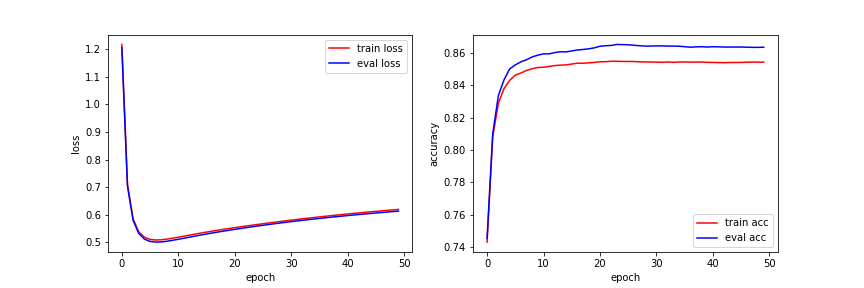
\includegraphics[width=1\textwidth]{50hidden1.png}
        \caption{Loss and accuracy plots for a neural network with a single 50-unit hidden layer. 
        The network was trained over 50 epochs. The achieved test loss and accuracy were 0.575 and 0.864, respectively.}
    \end{figure}
    \item[(b)] Number of units in the hidden layer was changed to 20 and 70 and the model was evaluated as in (a). The results appear in Figures 2 and 3, respectively.
    \begin{figure}[h!]
        \centering
        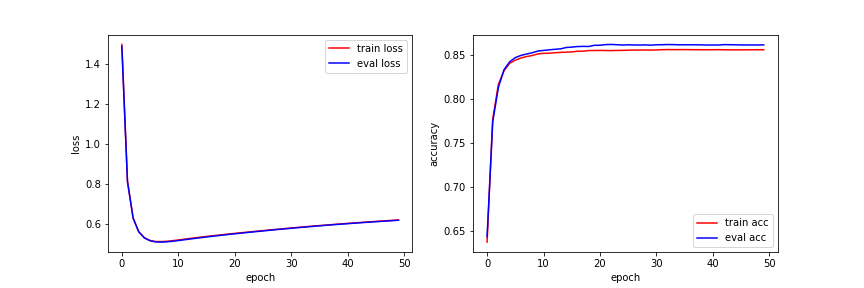
\includegraphics[width=1\textwidth]{20hidden1.png}
        \caption{Loss and accuracy plots for a neural network with a single 20-unit hidden layer. 
        The network was trained over 50 epochs. The achieved test loss and accuracy were 0.584 and 0.864, respectively.}
    \end{figure}
    \begin{figure}[h!]
        \centering
        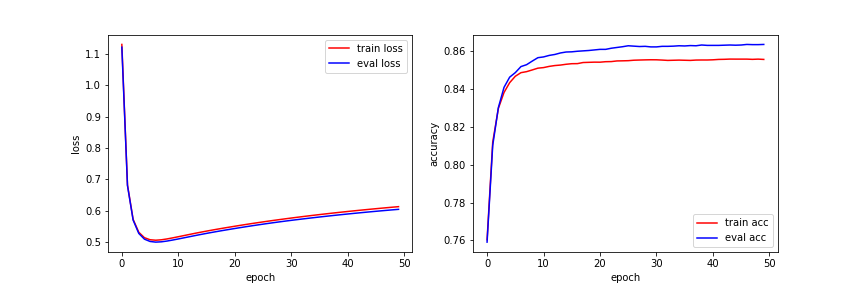
\includegraphics[width=1\textwidth]{70hidden1.png}
        \caption{Loss and accuracy plots for a neural network with a single 70-unit hidden layer. 
        The network was trained over 50 epochs. The achieved test loss and accuracy were 0.569 and 0.864, respectively.}
    \end{figure}
    \item[(c)] Next, a second hidden layer was introduced and the model performance was evaluated for different layer sizes. The results for the best model appear in Figure 4.
    \begin{figure}[h!]
        \centering
        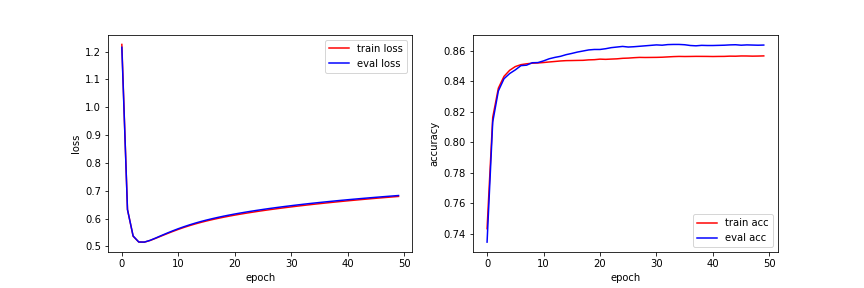
\includegraphics[width=1\textwidth]{300hidden1100hidden2.png}
        \caption{Loss and accuracy plots for a neural network with two hidden layers (300 and 100 units, repspectively). 
        The network was trained over 50 epochs. The achieved test loss and accuracy were 0.635 and 0.865, respectively.}
    \end{figure}
    \item[(d)] Now, we evaluate the performance of a model with 3 hidden layers containing 500, 300, and 100 units, respectively.
    The results are shown in Figure 5.
    \begin{figure}[h!]
        \centering
        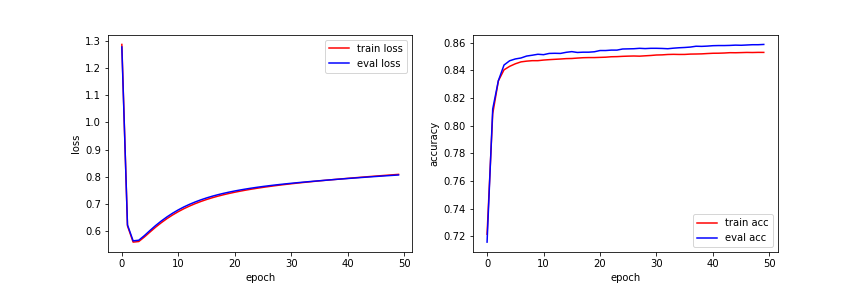
\includegraphics[width=1\textwidth]{500hidden1300hidden2100hidden3.png}
        \caption{Loss and accuracy plots for a neural network with three hidden layers (500, 300, and 100 units, repspectively). 
        The network was trained over 50 epochs. The achieved test loss and accuracy were 0.765 and 0.862, respectively.}
    \end{figure}
    A model with the same architecture was trained with a smaller learning rate (0.001 instead of 0.01), and the results can be seen in Figure 6.
    \begin{figure}[h!]
        \centering
        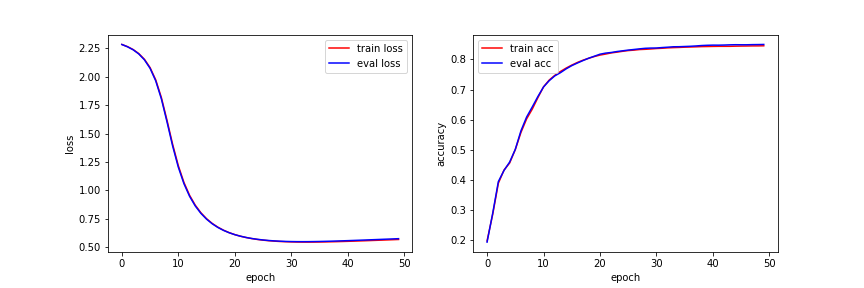
\includegraphics[width=1\textwidth]{500hidden1300hidden2100hidden3_lr0001.png}
        \caption{Same as in Figure 5 but with a smaller learning rate (0.001 instead of 0.01). The achieved test loss and accuracy were 0.544 and 0.855, respectively.}
    \end{figure}
\end{enumerate}

\end{document}
